

\section{HU4 Pantalla de confirmación de eliminación}

Si en la pantalla de la figura 4.5 \emph{"Pantalla de visualización"}, en el campo de “Selección” se selecciona uno o varios alumnos y se procede a presionar el botón Eliminar, mostrará un mensaje de confirmación, dando a conocer los datos del alumno a borrar: Nombre y Apellido junto con su matrícula. \\
La ventana emergente “Eliminar” tendrá 2 botones, siendo las opciones “Si” y “No”.
Una vez que se confirme o cancele la acción, regresara a la pantalla 4.5 \emph{"Pantalla de visualización"}

\begin{figure}[h]
	\centering
	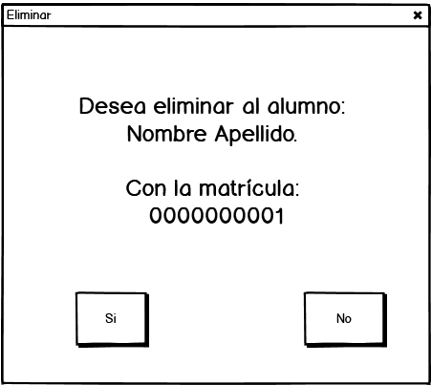
\includegraphics[scale=0.5]{./HistoriasUsuario/imagenes/IHU7.png}
	\caption{Pantalla de confirmación de eliminación}
\end{figure}
